\section{Methods}
\label{sec:methods}

% almost finished

\subsection{Data Prosessing}
\label{subsec:data_processing}

% almost finished

The Challenge did not provide ECG images directly for method development. Instead, it offered a tool \cite{Shivashankara_2024_ECG} to generate ECG images from ECG signals. We utilized this tool on the PTB-XL dataset \cite{wagner2020ptb_xl} and generated a total of 21,799 synthetic ECG images for our method development. Additionally, the PTB-XL+ dataset \cite{Strodthoff_2023} was used to generate classification labels for the ECG images.

The image generation setup included augmentations such as random Gaussian noise, random color temperature adjustments, and distortions including handwritten notes, wrinkles, and creases. Bounding boxes for the printed ECG waveforms and lead names, along with the plotted pixel coordinates of the ECG waveforms, were recorded in metadata files alongside the generated images. These supplementary data were used to:
\begin{itemize}
\item[(1)] Train the object detection model to detect the bounding boxes of the ECG waveforms and lead names in the ECG images, thus identifying the region of interest (ROI) for subsequent ECG signal extraction.
\item[(2)] Train the segmentation model to digitize the ECG waveforms from the images.
\end{itemize}

The PTB-XL dataset assigned a ``strat\_fold'' property (with values 1-10) to each record, which we used to split the dataset into training, and validation sets. The validation set has ``strat\_fold'' values 10, as recommended by the PTB-XL dataset, serving for model selection and hyperparameter tuning. The training set comprises the remaining records.

\begin{figure*}[!ht]
\centering
\begin{tikzpicture}[
node distance=1.2cm,
>={Triangle[angle=60:1pt 2]},
shorten >= 2pt,
shorten <= 2pt,
arrow/.style={
    ->,
    arrowblue,
    line width=5pt
}
]
\ImageNode[label={95:ECG Image}]{raw}{width=0.2\textwidth}{images/00666_hr-0.png}
\ImageNode[label={-90:Detected Boxes}, below right = 0.8cm and 1.35cm of raw.south east, anchor = south east]{bbox}{width=0.2\textwidth}{images/image_with_detected_boxes.pdf}
\ImageNode[label={-90:Extracted ROI}, right=of bbox]{roi}{width=0.2\textwidth}{images/ROI-example.pdf}
\ImageNode[label={-90:Segmented Waveforms}, below right=-0.2cm and 1.3cm of roi]{seg}{width=0.2\textwidth}{images/ROI_with_predicted_mask.png}
\node[above=of seg] (sig) {\textbf{Digitized 12-Lead Signal}};
\node[above=of roi] (cls) {\textbf{Predicted Classes}};
\ImageNode[above=0.1cm of sig]{sigch0}{width=0.2\textwidth}{images/ecg_eg_bare_ch0.pdf}
\begin{scope}[on background layer]
% \ImageNode[above right = 0.3cm and 0.3cm of sigch0.south west, anchor = south west]{sigch1}{width=0.2\textwidth}{images/ecg_eg_bare_ch1.pdf}
\node[rotate=45, above right=-0.4cm and 0.1cm of sigch0.north] (dots) {\huge $\cdots$};
\ImageNode[above right=-0.05cm and 0.3cm of dots.north, anchor=south]{sigchn}{width=0.2\textwidth}{images/ecg_eg_bare_ch1.pdf}
\end{scope}

\draw[arrow] (bbox) -- (roi);
\draw[arrow] (roi) -- (seg);
\draw[arrow] (seg) -- (sig);
\draw[arrow] (roi) -- (cls);
\draw[arrow] ([xshift=0.4cm]raw.north) to[out=30, in=90] ([xshift=-0.4cm]bbox.north east);

\draw[rounded corners] ([shift={(-0.4cm,1.2cm)}]raw.north west) rectangle ([shift={(0.5cm,-0.6cm)}]seg.south east);

\end{tikzpicture}

\caption{The multi-stage framework for simultaneous digitization and classification of ECG images.}
\label{fig:multi-stage-framework}
\end{figure*}

\subsection{The Multi-Stage Framework}
\label{subsec:multi_stage_framework}

% almost finished

To simultaneously digitize and classify ECG images, we propose a multi-stage framework, as illustrated in Figure \ref{fig:multi-stage-framework}. The framework comprises three deep learning-based modules: object detection, segmentation, and classification.

The object detection module identifies the bounding boxes of the ECG waveforms and lead names in the ECG images, thereby determining the region of interest (ROI) for subsequent ECG signal extraction and classification. This module constitutes the first stage of the framework.

The segmentation module extracts a mask of the ECG waveforms from the ROI, which is then transformed into digitized values based on the pixel coordinates of the predicted mask. The bounding boxes obtained from the object detection module are also used to separate the ECG waveforms at different horizontal positions. In cases where the bounding boxes overlap, which commonly occurs when the ECG signals have large amplitudes, we employ a 4-cluster K-means algorithm on the y-coordinates of the predicted mask to locate the isoelectric line of the ECG waveforms and then perform the separation. Concurrently, the classification module predicts the classes of the ECG waveforms from the ROI. These two modules together constitute the second stage of the framework.

\subsection{Model Selection}
\label{subsec:model_selection}

% almost finished

We present our criteria for selecting the deep learning models for the three modules discussed in Section \ref{subsec:multi_stage_framework}. The models are chosen based on their performance, efficiency, and compatibility with ECG image data. After evaluating several models, we choose the following models for the three modules:
\begin{itemize}
\item[(1)] Object Detection: A DETR model \cite{carion2020DETR} with a ResNet-50 backbone \cite{resnet}.
\item[(2)] Classification: A lightweight ConvNeXt model \cite{Liu_2022_ConvNeXt} of ``nano'' size.
\item[(3)] Segmentation: A U-Net model \cite{unet}.
\end{itemize}
The object detection model and the classification model are trained from a pre-trained model loaded from Huggingface's model hub \cite{wolf-etal-2020-transformers}, while the segmentation model is trained from scratch. The models are implemented and trained using the ``torch\_ecg'' library \cite{torch_ecg_paper}. The sizes in terms of the number of trainable parameters of the selected models are listed in Table \ref{tab:model_num_params}.

\begin{table}[!htp]
\centering
% requires packages boldline, multirow
\setlength\tabcolsep{2pt}
\begin{tabular}{@{\extracolsep{6pt}}c|ccc@{}}
\hlineB{3.5}
& ConvNeXt-nano & DETR-ResNet-50 & U-Net \\
\hlineB{2}
\# Params & $15$M & $41$M & $31$M \\
\hlineB{3.5}
\end{tabular}
\caption{Number of trainable parameters in the models.}
\label{tab:model_num_params}
\end{table}


It is important to note that for the classification model, using an oversized model may not improve the performance and can even degrade it due to overfitting. Therefore, we opted for a lightweight model to balance performance and efficiency. The evaluation metrics (in terms of F1 score) of different sizes of ConvNeXt models on the left-out validation set, along with their number of trainable parameters, are presented in Table \ref{tab:clf_selection}.

\begin{table}[!htp]
\centering
% requires packages boldline, multirow
\setlength\tabcolsep{2pt}
\begin{tabular}{@{\extracolsep{6pt}}c|cccc@{}}
\hlineB{3.5}
\multirow{2}{*}{Threshold} & \multicolumn{4}{c}{size of the ConvNeXt model} \\ 
\cline{2-5}
& \textbf{nano} & base & large & nano (head only) \\
\hlineB{2}
$0.5$ & $0.287$ & $0.243$ & $0.208$ & $0.216$ \\
$0.7$ & $0.344$ & $0.284$ & $0.207$ & $0.213$ \\
$0.9$ & $\mathbf{0.428}$ & $0.382$ & $0.205$ & $0.237$ \\
$0.95$ & $\mathbf{0.450}$ & $\mathbf{0.448}$ & $0.197$ & $0.218$ \\
\hlineB{2}
\# Params & $15$M & $88$M & $197$M & $0.3$M \\
\hlineB{3.5}
\end{tabular}
\caption{Evaluation metrics of different sizes of ConvNeXt models. The values are F1 scores on the left-out validation set. The threshold refers to the probability threshold for the multi-label classification task. ``head only'' refers to the ConvNeXt model with backbone weights frozen. The last row shows the number of trainable parameters in each model.}
\label{tab:clf_selection}
\end{table}


The DETR model achieved a mean average precision (mAP) of $0.90$ and the U-Net model achieved a Dice coefficient of $0.73,$ both on the left-out validation set.

\subsection{Loss Functions}
\label{subsec:loss_functions}

% almost finished

\begin{figure}[!htp]
\centering
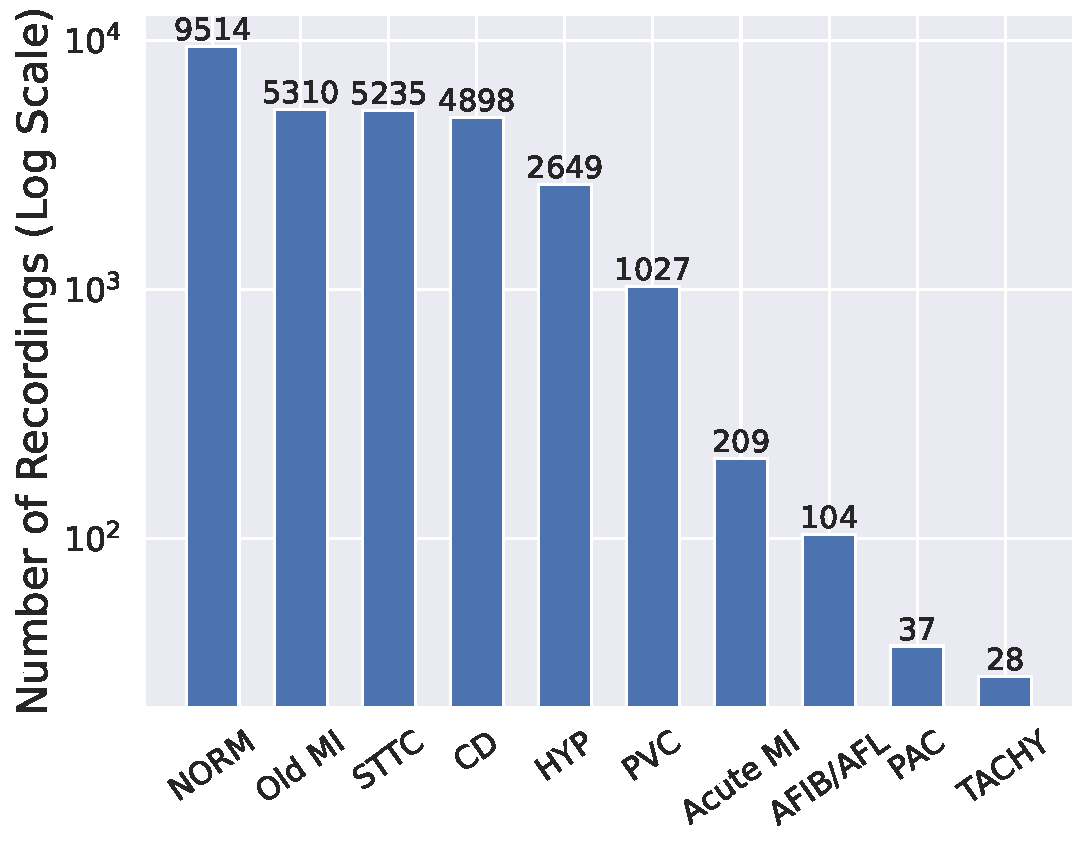
\includegraphics[width=\linewidth]{images/data_distribution.pdf}
\caption{Data distribution of the PTB-XL dataset. Labels are generated from the PTB-XL+ dataset. Abbreviations: NORM, Normal; OLD MI, Old Myocardial Infarction; STTC, ST/T Changes; CD, Conduction Disturbances; HYP, Hypertrophy; PVC, Premature Ventricular Complex; Acute MI, Acute Myocardial Infarction; AFIB/AFL, Atrial Fibrillation/Atrial Flutter; PAC, Premature Atrial Complex; TACHY, Tachycardia.}
\label{fig:data-distribution}
\end{figure}

Since the data (label) distribution for the classification problem is highly imbalanced as can be observed in Figure \ref{fig:data-distribution}, and also considering that this is a multi-label problem, we adopted the asymmetric loss \cite{ridnik2021asymmetric_loss} as the loss function. The asymmetric loss is defined in Equation \eqref{eq:asymmetric_loss}.
\begin{equation}
\label{eq:asymmetric_loss}
\begin{array}{ll}
& L = -y \cdot (1-p)^{\gamma_{+}} \log(p) \\
& \phantom{L = } - (1-y) \cdot (p_m)^{\gamma_{-}} \log(1-p_m), \\
\text{where} & p_m = \max(p - m, 0),
\end{array}
\end{equation}
where $y$ is the ground truth label, $p$ is the predicted probability, $m$ is the probability margin, and $\gamma_{+}$ and $\gamma_{-}$ are the positive and negative focusing parameters, respectively. The margin $m$ and the focusing parameters $\gamma_{+}$ and $\gamma_{-}$ are hyperparameters that can be tuned. We set $\gamma_{+} = 1,$ $\gamma_{-} = 4,$ and $m = 0.05$ in our experiments.

For the segmentation task, considering that the ECG waveforms occupy only a small portion of the image, we used the binary cross-entropy loss multiplied by a weight mask to balance the loss contribution from different parts of the ECG waveforms. The weight mask is the sum of multiple dilations (for example of iterations $2, 4, 6, 8$) of the binarized ground truth mask. An example of the weight mask is shown in Figure \ref{fig:weight-mask}.

\begin{figure}[!htp]
\centering
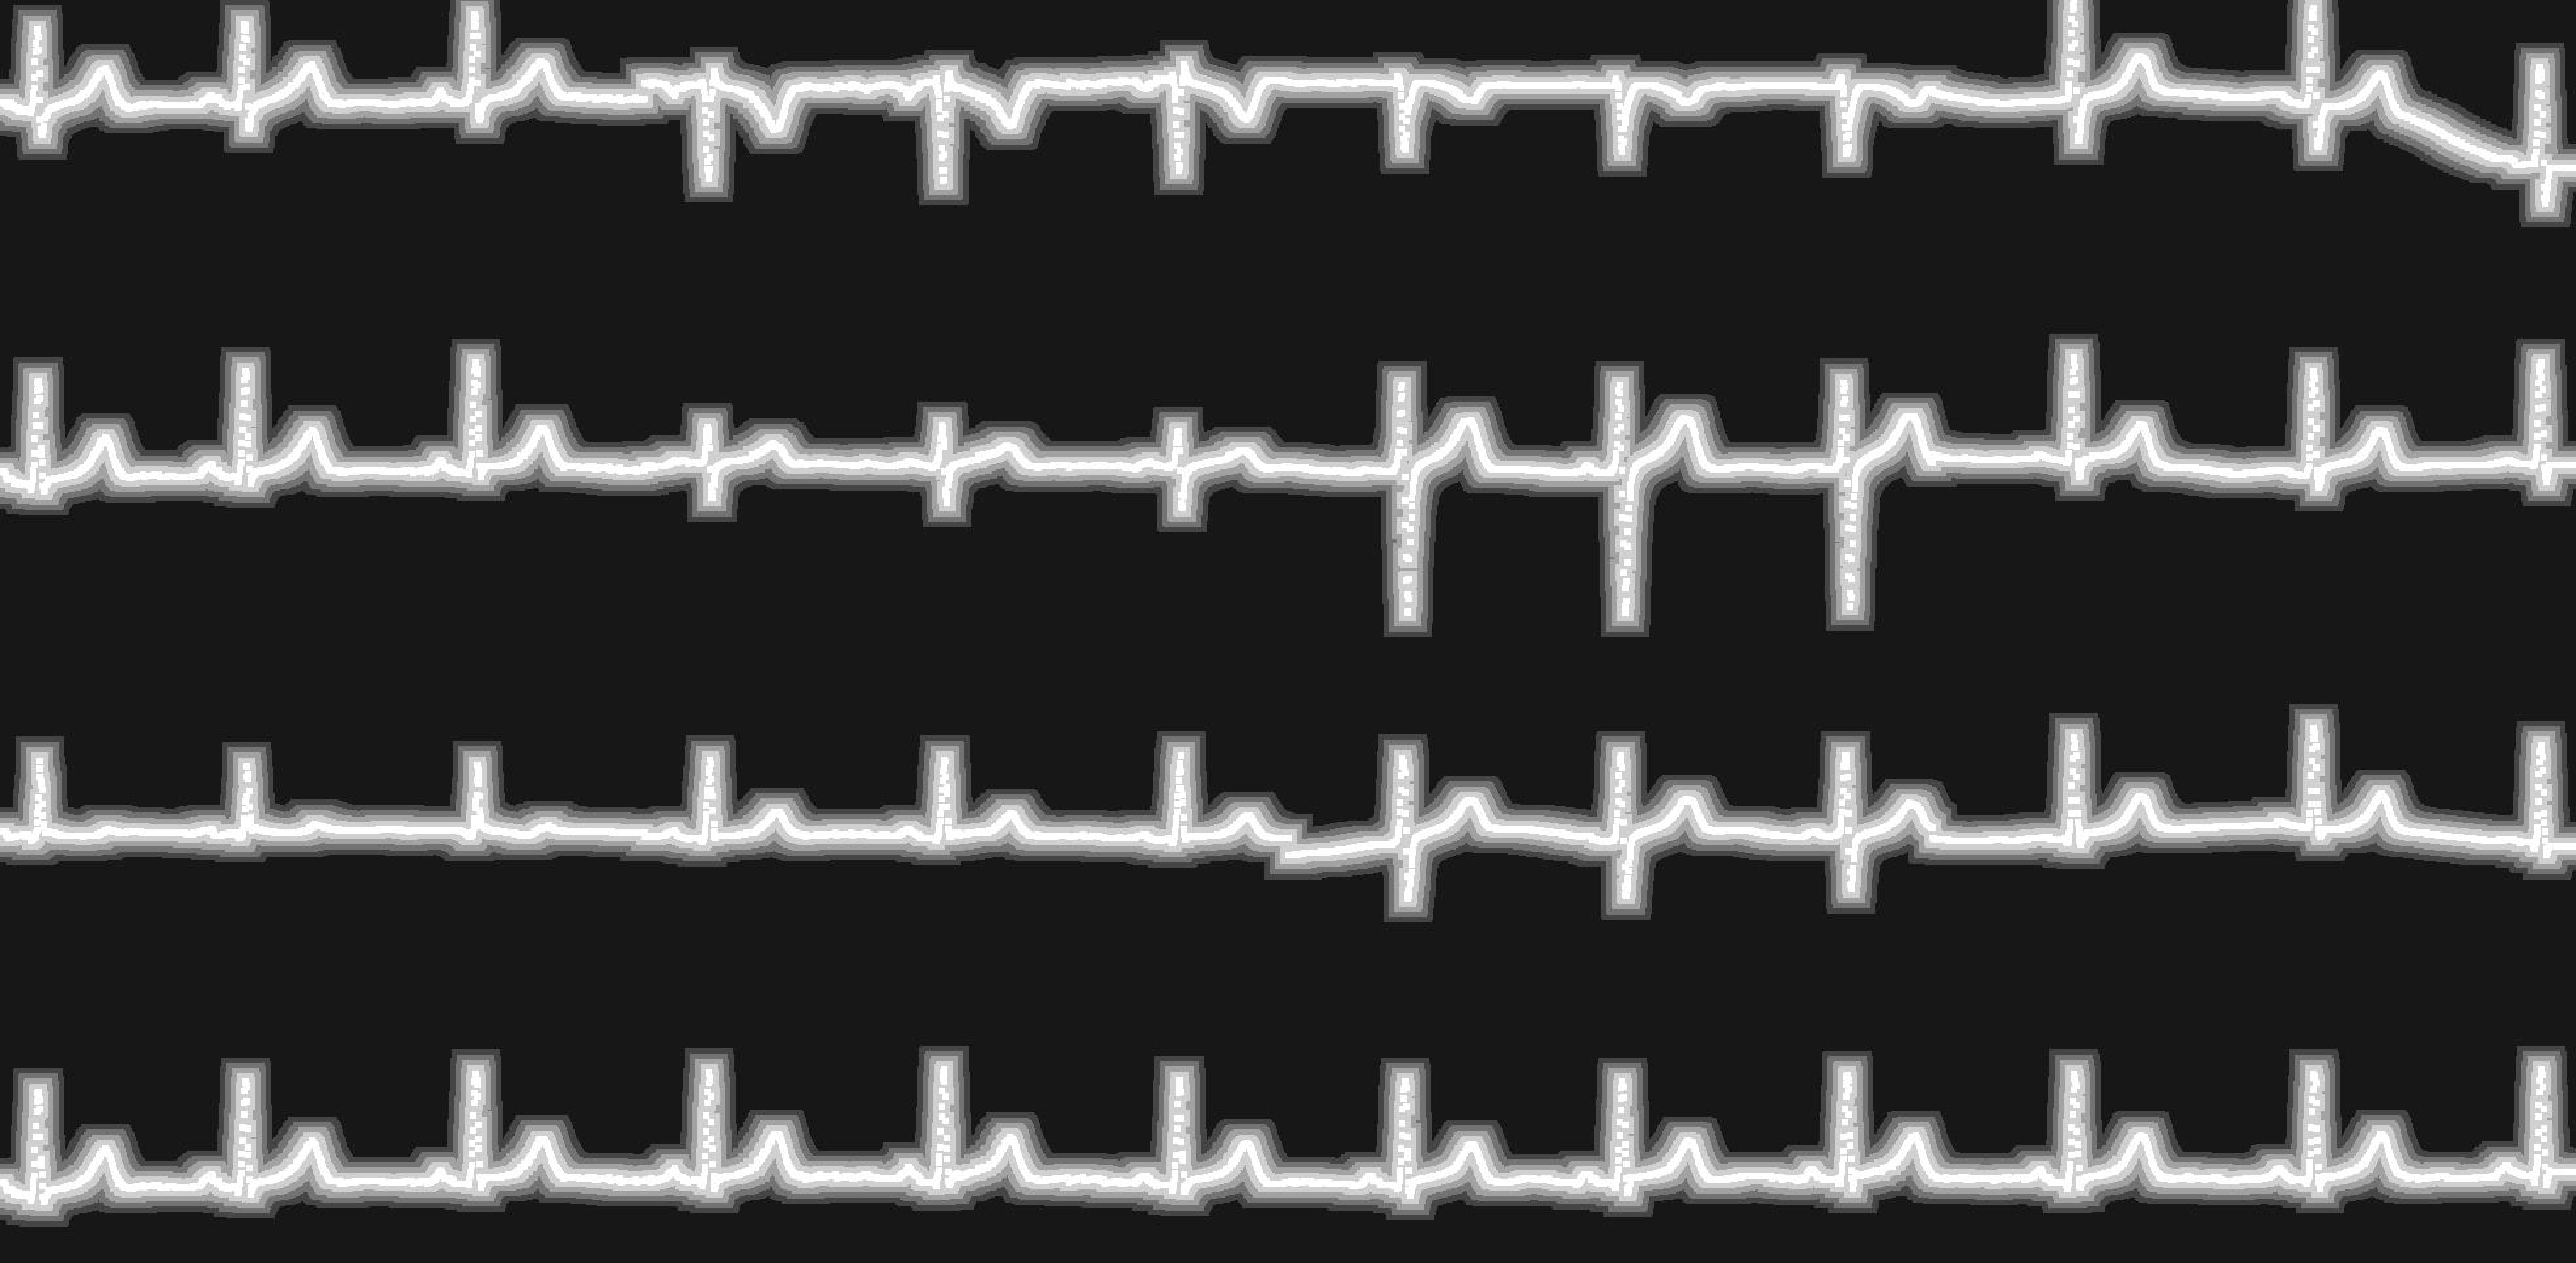
\includegraphics[width=\linewidth]{images/weight-mask.pdf}
\caption{An example of the weight mask for the segmentation loss function.}
\label{fig:weight-mask}
\end{figure}

For the object detection task, we used the standard DETR loss function, which is a linear combination of the cross-entropy loss of the bounding box class predictions (coefficient $1$) and the bounding box coordinate regression loss ($L1$ loss with coefficient $5$ and generalized IoU loss with coefficient $2$).
